\chapter{Les profils UML}
%OMG Unified Modeling LanguageTM (OMG UML),Superstructure
\label{profils-UML.sect}
\section{Le langage de modélisation UML}
\gls{uml} est un langage de modélisation standardisé permettant de créer des diagrammes.
Ces diagrammes permettent de visualiser, spécifier, construire et documenter des logiciels, des systèmes et des processus d'affaire.
UML utilise des notations graphiques pour exprimer le design et l'architecture de projets logiciels.
Les spécifications du standard UML sont en ligne sur le site de l'OMG (Object Management Group)  \cite{OMG_UML}.
Dans la figure \ref{fig.uml_struc} sont représentés les diagrammes de structure proposés par UML.
Dans la figure \ref{fig.uml_comp} sont proposés les diagrammes de comportement proposés par UML.

\begin{figure}[H]
    \centering
    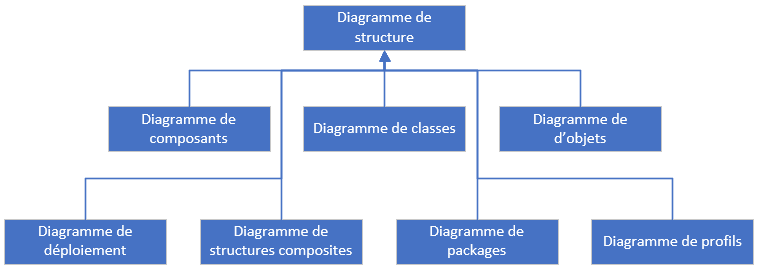
\includegraphics[width=12cm]{10_img/chap4/structure.PNG}
    \caption{Diagrammes de structure dans UML \cite{OMG_UML}}
    \label{fig.uml_struc}
\end{figure}

\begin{figure}[H]
    \centering
    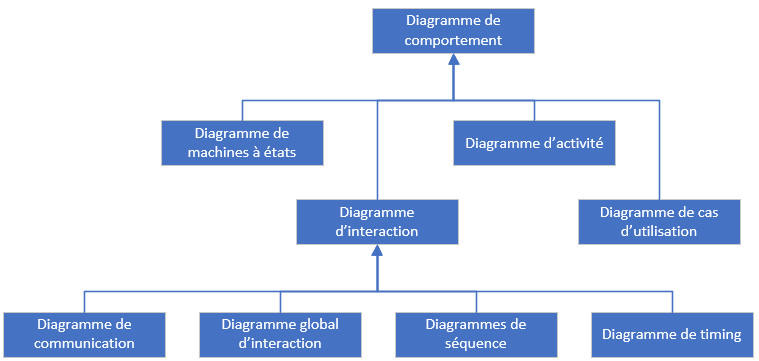
\includegraphics[width=12cm]{10_img/chap4/comportement.PNG}
    \caption{Diagrammes de comportement dans UML \cite{OMG_UML}}
    \label{fig.uml_comp}
\end{figure}

UML est un langage de modélisation connu et largement documenté dans le domaine de l'informatique.
Nous nous concentrerons plus particulièrement à définir les notions nécessaires à la compréhension des mécanismes et des éléments composant les profils UML.

\section{Le diagramme de profil UML}
Un profil UML est une forme de diagramme structurel décrit dans le standard UML.
Il permet d'étendre les mécanismes d'UML afin d'adapter les diagrammes et leur contenu à un domaine (ex : domaines d'activité) ou une plateforme particulière (ex : .NET, J2EE).

Les extensions qu'un profil appliquées au langage UML permettent d'ajouter des caractéristiques aux éléments standards d'UML.
Elles ne permettent pas de retirer les caractéristiques des éléments pour ne pas aller à l'encontre de la sémantique standard d'UML.
Le profil se compose  de stéréotypes de tagged values et de contraintes qui s'appliquent aux éléments des modèles UML tels que les classes, les attributs, les opérations et les activités.


\subsection{stereotypes}
Les stéréotypes permettent d'appliquer des extensions aux métaclasse UML.
Il permettent d'ajouter des termes spécifiques de vocabulaire à un diagramme.
Un stéréotype s'applique à un objet UML permettant ainsi de le rendre spécifique à un domaine en y appliquant des propriétés spécifiques.

\subsection{extensions}
link entre metaclass et stereotype


\subsection{contraintes}
ex : un stereotype peut generaliser ou specialiser un autre stereotype


\subsection{tagged values}


\subsection{Image}


\subsection{reponse a la pb}
